%!TEX root = ../Touch Based Idris.tex
\section{Third Usability Iteration}
In this section we first describe our latest design with reference to the
recommendations from earlier sections. Then we discuss how the next iteration
of usability testing should be carried out.

We have thought long and hard about the consequences of making our editor more
structured. On one hand there would be a lower risk of the programmer making  syntax errors, but on the other hand there would not be as much freedom to approach
the programming task in the way the individual prefers.

We have seen how the heavy overload of touch-gestures in the Lisping editor makes it hard to use
the interface. So far, in the IdrisTouch editor, we seem to have the same
problem. If the user wants to case split a term, double tapping it is required,
but that gesture is actually already in use by the text field that shows the
term. The result of the double tap is both case splitting the term and marking
its text.

One tempting solution would be to make the editor much more structured and only
have one text field in the whole interface. This text field would be placed in
the context popover and only allow the user to search the current context. The only way to add terms to the editor would be to choose a term in the list of applicable terms in the context popover (See Figure \ref{fig:new_design_popover}). This
would ensure that we could incorporate all the touch gestures we needed for
manipulating the program structure. No conflicts with text fields would occur.

\begin{figure}
	\centering
		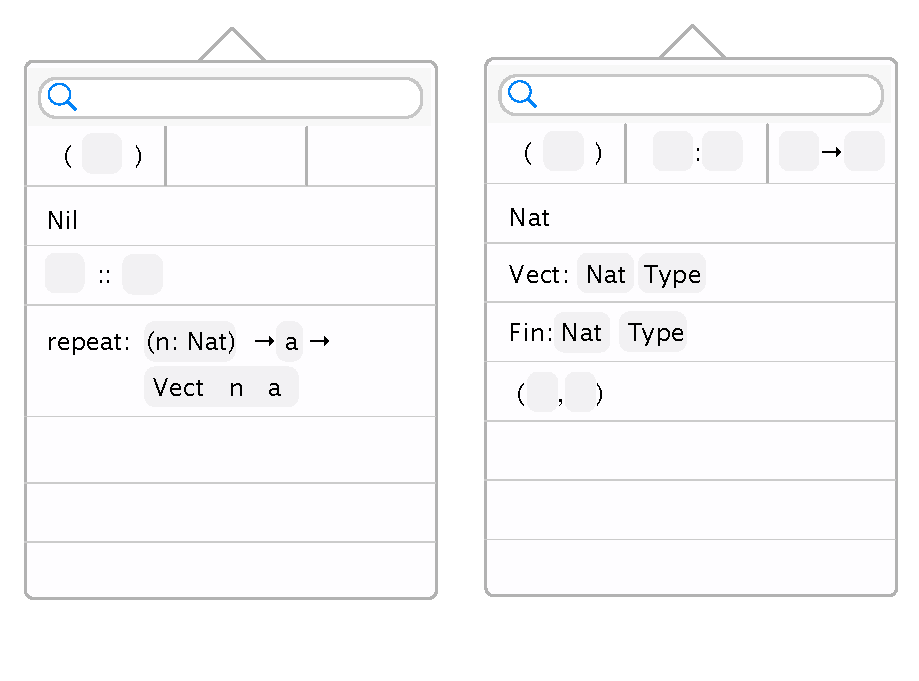
\includegraphics[width=110mm]{diagrams/final_design_popover.pdf}
	\caption{The context popover. Left: How it looks when a \texttt{Vect} is
	expected. Right: How it looks when defining a new type constructor.}
\label{fig:new_design_popover}
\end{figure}

The problem with this approach is the lack of flexibility for the programmer.
Strictly structured editors dictate a certain way of programming. The solution
that we found appropriate, was to move towards a somewhat more structured editor that holds program structure but lets the user edit code in free text, like TouchDevelop. We allow programmers
to build their program in a structured way by searching for terms in the
content popover, but editing terms is also allowed in free text.

This means that terms can have two states. Either they are being edited or they are not. Entering the edit mode is done by double tapping the term and has the effect of making the UI element showing the element into a regular text field. This means that we will have to find another touch-gesture for case-splitting and meta variable solving
that have used double tap so far. Reserving
the double tap
gesture to activate the edit mode removes all of the gesture overloads we have
had so far. Now we can have dragging, flicking and holding touch-gestures
without any conflicts. More on the new set of gestures in Section \ref{subsec:new_design_data_dec} and \ref{subsec:new_design_function_dec}.

\subsection{Managing Program Structure}
Figure \ref{fig:new_design_nothing_in_focus} shows two top-level declarations
where none of them are in focus. In this state the programmer can get a clear
overview of the program without any clutter. Tapping anywhere on e.g.
the data declaration takes the user to the state seen in Figure \ref{fig:new_design_data_in_focus},
where the elements of the declaration are bigger and easier to tap. The check mark button
removes focus from the current declaration and should help mitigate Re7 by
giving the user a clear way to indicate that he is done with editing. Tapping
other top-level declarations will switch the current editable declaration to
non-editable and switch the tapped top-level declaration to editable.

\begin{figure}
	\centering
		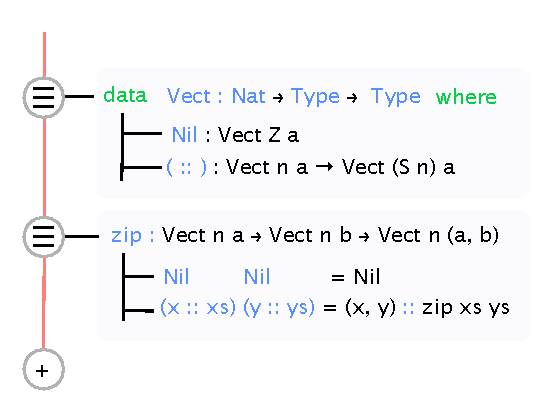
\includegraphics[width=100mm]{diagrams/final_design_nothing_in_focus.pdf}
	\caption{The new design with no particular declarations in focus}
\label{fig:new_design_nothing_in_focus}
\end{figure}

\begin{figure}
	\centering
		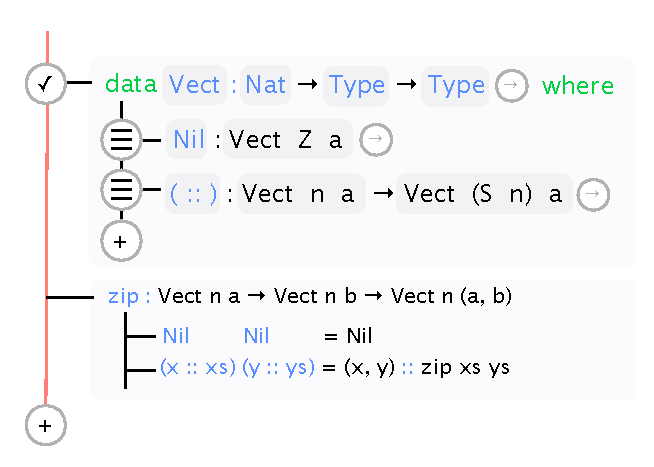
\includegraphics[width=100mm]{diagrams/final_design_top_dec_in_focus.pdf}
	\caption{The new design with a data declarations in focus. The code becomes
	bigger and easier to tap}
\label{fig:new_design_data_in_focus}
\end{figure}

\begin{figure}
	\centering
		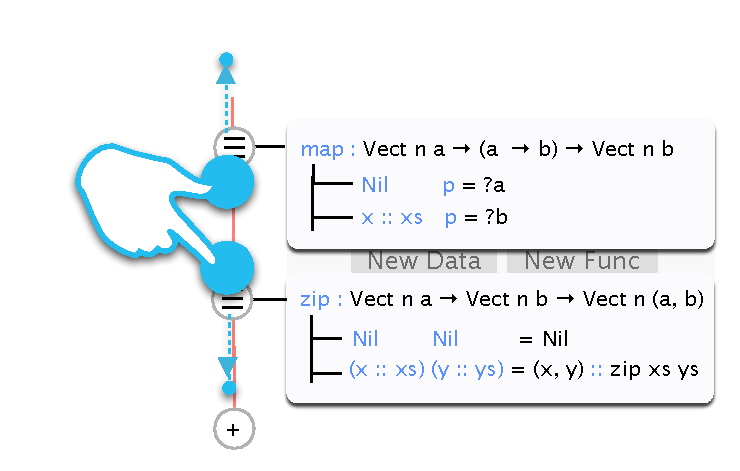
\includegraphics[width=110mm]{diagrams/new_function_reverse_pinch.pdf}
	\caption{When reverse pinching two adjacent handles for top-level
	declarations, a new top-level declaration appears between the old ones.}
\label{fig:new_function_reverse_pinch}
\end{figure}

We have decided to keep our original design for creating new top-level
declarations. Either, the programmer can use the [+] button at the bottom of
the program, or he can reverse-pinch two adjacent top-level declarations to
create a new one between them. This also works for creating constructors
between existing constructors in data declarations.

Now that the representation of a term is no longer overloaded with conflicting
gestures, we can incorporate drag-to-rearrange. Figure \ref{fig:design_drag_to_garbage}
shows an example of this behavior. When the user begins to drag a term, it pop
out of its current position, and can be rearranged with other terms on the same
line. Also, while the user is dragging the term, a trash icon appears in the
upper right corner of the screen, to indicate that it can be deleted. Experienced users can flick the term towards the trash icon, whereas novice users will just drag it nicely
the first couple of times.

\begin{figure}
	\centering
		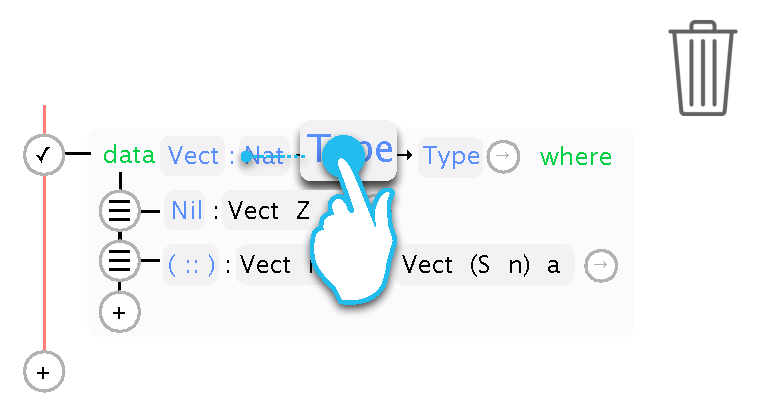
\includegraphics[width=110mm]{diagrams/design_drag_to_garbage.pdf}
	\caption{When reverse pinching two adjacent handles for top-level
	declarations, a new top-level declaration appears between the old ones.}
\label{fig:design_drag_to_garbage}
\end{figure}

\subsection{Data Declarations}
\label{subsec:new_design_data_dec}
We now incorporate a new (old) way of
declaring data, and it now resembles the textual Idris syntax. 

Looking at Figure \ref{subsec:new_design_data_dec}, the grayed out arrow buttons indicate that a new term can be added. When no
keyboard is present on the screen this is the only way to add new terms, but if
the keyboard is present, which means that a term is being edited, another term
can be added by using the similar arrow button found in the upper right corner
of the keyboard (see Figure \ref{fig:design_keyboard}). This keyboard has a
Texstastic-inspired way of inputting all of the special characters allowed in
Idris. This design solves requirement F-10.

\begin{figure}
	\centering
		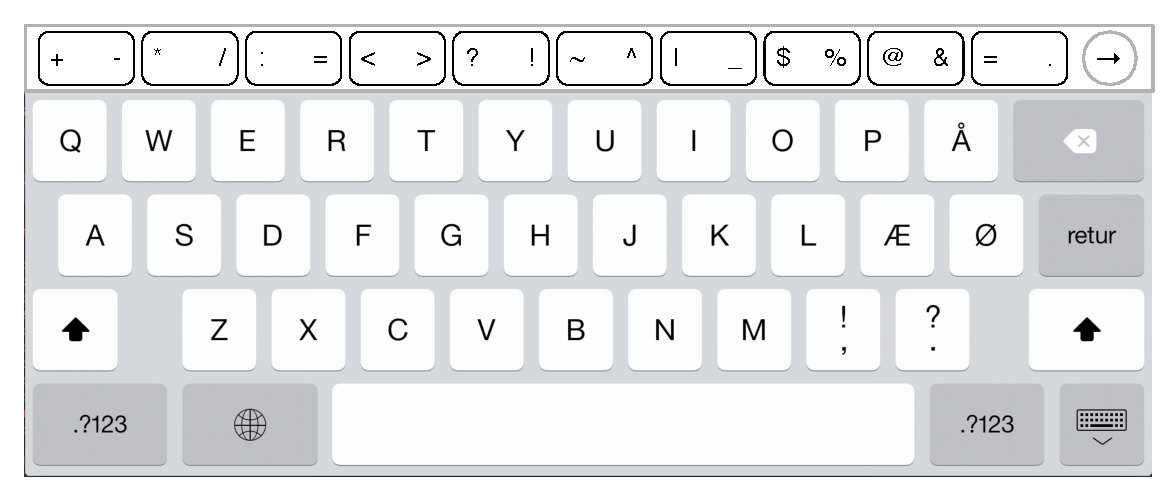
\includegraphics[width=115mm]{diagrams/design_keyboard.pdf}
	\caption{The Textastic-inspired keyboard with the special characters that
	Idris allows for operator definition. The right-most arrow button creates new
	terms.}
\label{fig:design_keyboard}
\end{figure}



\subsection{Function Declarations}
\label{subsec:new_design_function_dec}
The function declarations work much the same way as the data declarations
except for the extra support for initial pattern match creation, case splitting
and meta variable solving.

The initial pattern match creation is still done by pressing the [+] button to
add a new clause. Case splitting can no longer be done by double tapping a
term, as this would toggle it to edit mode. Instead, the user drags the term
down and a new clause appears like it can be seen in Figure
\ref{fig:case_splitting}.

\begin{figure}
	\centering
		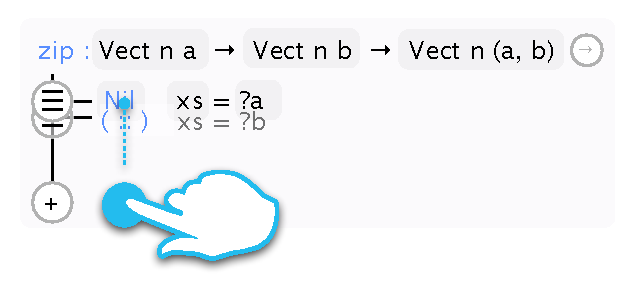
\includegraphics[width=100mm]{diagrams/design_case_splitting.pdf}
	\caption{Case splitting is done by dragging a term down until a new clause
	appears.}
\label{fig:case_splitting}
\end{figure}

Meta variable solving is managed in an even simpler way. If a term starts with
a question mark like in Figure \ref{fig:case_splitting} then a single tap will
tell the compiler to try and automatically solve the meta variable. Double
tapping it will as always make the term toggle to edit mode.



\subsection{Error Handling}







\subsection{Next Usability Iteration}
With this new design we feel that the user interface has reached a maturity
level where it is important to focus on the server-side for a while. In the
next usability test, the solution's edit-compile-test cycle should be tested to
a larger extent, and that requires a working back-end. The following usability
test cases assume that we have a working prototype with the new design
implemented as well as a working server that can serve compilation results.

The participants of the usability test should again be a mix of programmers
that are new to the platform and some that are not. Other than that, they
should be screened in the same way as in our second usability test (Section
\ref{sec:SecondUsabilityTest}).

What we specifically wish to test in this next usability test is:

\begin{enumerate}
	\item The flow when declaring new data types and functions. This includes the auto-completion feature and the context popover
	\item The understandability of the way we now declare data types
	\item The focus system, where only one top-level declaration is in focus at a
	time. Can users maneuver in and out of declarations in a fairly easy way?
	\item Editing right-hand sides that have already been added.
	\item Deleting terms by flicking them and rearranging them by dragging.
	\item Deleting top-level declarations, clauses, and constructors
\end{enumerate}

It does not make sense to draw up an exact usability test plan like the ones we have made in previous usability
at this point. We would need to have a working version of the solution before a precise test plan can be made. Also, the few points listed above could easily amount to more than 10 tasks, which is more than can be completed in an hour with a participant. For this reason we would have to prioritize the focus of the test, and that can only be done when we have the new solution in our hands and decide what features we are most confident about. 




